\documentclass[10pt,a4paper]{article}
\usepackage[utf8]{inputenc}
\usepackage[spanish]{babel}
\usepackage{amsmath}
\usepackage{amsfonts}
\usepackage{amssymb}
\usepackage{graphics}
\usepackage{graphicx}
\usepackage{xcolor}
\usepackage{listings}
\usepackage{csvsimple}
\usepackage{caption}
\usepackage{subcaption}
\usepackage[left=2cm,right=2cm,top=2cm,bottom=2cm]{geometry}

\setcounter{MaxMatrixCols}{20}

\renewcommand*\contentsname{Índice} %Nombre del indice

\begin{document}
\lstset{
	basicstyle=\footnotesize,
	extendedchars=true,
	literate={á}{{\'a}}1 {ã}{{\~a}}1 {é}{{\'e}}1 {ú}{{\'u}}1 {ó}{{\'o}}1,
	backgroundcolor=\color{black!5}
	}
	
\begin{titlepage}
	\centering
	{
\includegraphics[scale=0.5]{Logo_UGR.png}\par}
	\vspace{1cm}
	{\bfseries\Large Escuela T\'ecnica Superior de Ingeniería Informática y Telecomunicaciones \par}
	\vspace{2.5cm}
	{\scshape\Huge Pr\'actica 4: Programación Dinámica \par}
	\vspace{3cm}
	{\itshape\Large Doble Grado Ingeniería Informática y Matemáticas}
	\vfill
	{\Large Autores: \par}
	{\Large Jose Alberto Hoces Castro\par}
	{\Large Javier Gómez López \par}
	{\Large Moya Mart\'in Castaño \par}
	\vfill
	{\Large Mayo 2022 \par}
\end{titlepage}

\thispagestyle{empty}
\null
\vfill

%%Información sobre la licencia
\parbox[t]{\textwidth}{
  
\includegraphics[scale=0.05]{by-nc-sa.png}\\[4pt]
  \raggedright % Texto alineado a la izquierda
  \sffamily\large
  {\Large Este trabajo se distribuye bajo una licencia CC BY-NC-SA 4.0.}\\[4pt]
  Eres libre de distribuir y adaptar el material siempre que reconozcas a los\\
  autores originales del documento, no lo utilices para fines comerciales\\
  y lo distribuyas bajo la misma licencia.\\[4pt]
  \texttt{creativecommons.org/licenses/by-nc-sa/4.0/}
}

\newpage

\tableofcontents

\newpage

\section{Introducción}

El objetivo de esta práctica es aprender a implementar y utilizar algoritmos que utilizan la técnica de programación dinámica. Para ello hemos tenido que resolver el siguiente ejercicio:\\

\textbf{Enunciado.} \textit{Dos hermanos fueron separados al nacer y mediante un programa de televisión se han enterado que podrían ser hermanos. Ante esto, los dos están de acuerdo en hacerse un test de ADN para verificar si realmente son hermanos.}\\
\\
Dadas las 2 entradas:\\
\\
\textbf{PRIMERA} \\
Hermano 1 - abbcdefabcdxzyccd \\
Hermano 2 - abbcdeafbcdzxyccd \\
\\
\textbf{SEGUNDA}\\
Hermano 1 - $010111000100010101010010001001001001$\\
Hermano 2 - $110000100100101010001010010011010100$\\

\begin{itemize}
	\item Deben encontrar el \% de similitud que existe entre estos posibles hermanos, como es un ejemplo lo haremos para 2 entradas posibles.
	\item Dar las salidas (secuencia más larga) de las 2 entradas.
	\item Dar la matriz de los cálculos de la primera entrada.
\end{itemize}

\section{Requisitos de la Progamación Dinámica}
Como ya sabemos, la programación dinámica se aplica en cuatro fases que vamos a identificar:

\begin{itemize}
	\item \textbf{Naturaleza n-etápica:} Para hallar la mayor subsecuencia entre dos secuencias dadas, comenzamos hallando la subsecuencia más larga para el primer carácter de las dos secuencias, después la más larga teniendo en cuenta los dos primeros caracteres, y así hasta tener en cuenta los caracteres de ambas secuencias en su totalidad.
	\item \textbf{Verificación del POB (Principio de Optimalidad de Bellman):} Sea $ s_i, s_{i+1},...., s_{i+k}, s_j$ la mayor subsecuencia del índice \(i\) hasta el \(j\).
	Comenzando en el elemento $s_i$ correspondiente al índice $i$, entonces hemos encontrado, el siguiente elemento común en ambas entradas, que es $s_{i+1}$. Por tanto, ahora necesitamos encontrar la mayor subsecuencia común entre el índice que le corresponde a $s_{i+1}$, es decir, $i+1$, llamémoslo $l$, y el índice $j$. Es claro que entre $l$ y $j$ la subsecuencia $s_{i+1},...., s_{i+k}$ debe ser la de mayor longitud. De no serlo, entonces existiría una subsecuencia $s_{i+1}, t_3, t4, ...., t_r, s_j$ con $r>k$ entre los índices l y j que sería de mayor longitud. Entonces, tendríamos que $s_i, s_{i+1}, t_3, t4, ...., t_r, s_j$ es una subsecuencia de mayor longitud que $ s_i, s_{i+1},...., s_{i+k}, s_j$ del índice $i$ al $j$.
	\item \textbf{Planteamiento de una recurrencia:} Para resolver este problema, vamos a hacer uso de una matriz de dimensión $n \cdot m$, siendo $n$ y $m$ las longitudes de las secuencias de nuestro problema: 
	
	1. Comenzaremos rellenando la primera fila y la primera columna de ceros.
	
	2. Rellenamos el resto de la matriz según el siguiente criterio:
	
	Si el carácter $i$ de la primera secuencia coincide con el carácter $j$ de la segunda secuencia, la casilla $<i,j>$ se rellenará con el valor de la casilla $<i-1,j-1>$ más $1$. Así, estamos teniendo en cuenta si ha habido coincidencias anteriormente a esos índices para poder formar la subsecuencia. En caso de no haber coincidencia entre esos índices, se toma el valor máximo entre los de las casillas $<i-1,j>$ y $<i,j-1>$, ya que debemos tener en cuenta las coincidencias que ha habido antes de esos índices a pesar de no haber coincidencia entre ellos.
	
	3. Por último, hallamos el máximo de la matriz (que estará situado en la última fila) deshaciendo el camino que hemos ido haciendo por las casillas y teniendo en cuenta si estamos en una posición de coincidencia o no.
	
	Gracias a esta forma de ir anotando las coincidencias que se van hallando entre ambas secuencias, estamos almacenando de forma numérica la secuencia más larga dados dos índices de ambas secuencias. En resumen, nuestra matriz se rellenará según la siguiente expresión:
	
	\[
	A(i,j)= \left\{ \begin{array}{lcc}
		0 &   si  &  \hspace{0.2cm} i=j=0 \\
		\\ max(A(i-1,j),A(i,j-1)) &  si  & x_i \neq y_j \hspace{0.2cm}\\
		\\ A(i-1,j-1) + 1 & si & x_i = y_j \hspace{0.2cm}
	\end{array}
	\right.
	\]
	
	Dado un ejemplo pequeño de secuencias, sean $<A,B,C,B,D,A,B>$ y $<B,D,C,A,B,A,E>$, la matriz usando nuestro algoritmo quedaría así:
	
	\begin{center}
		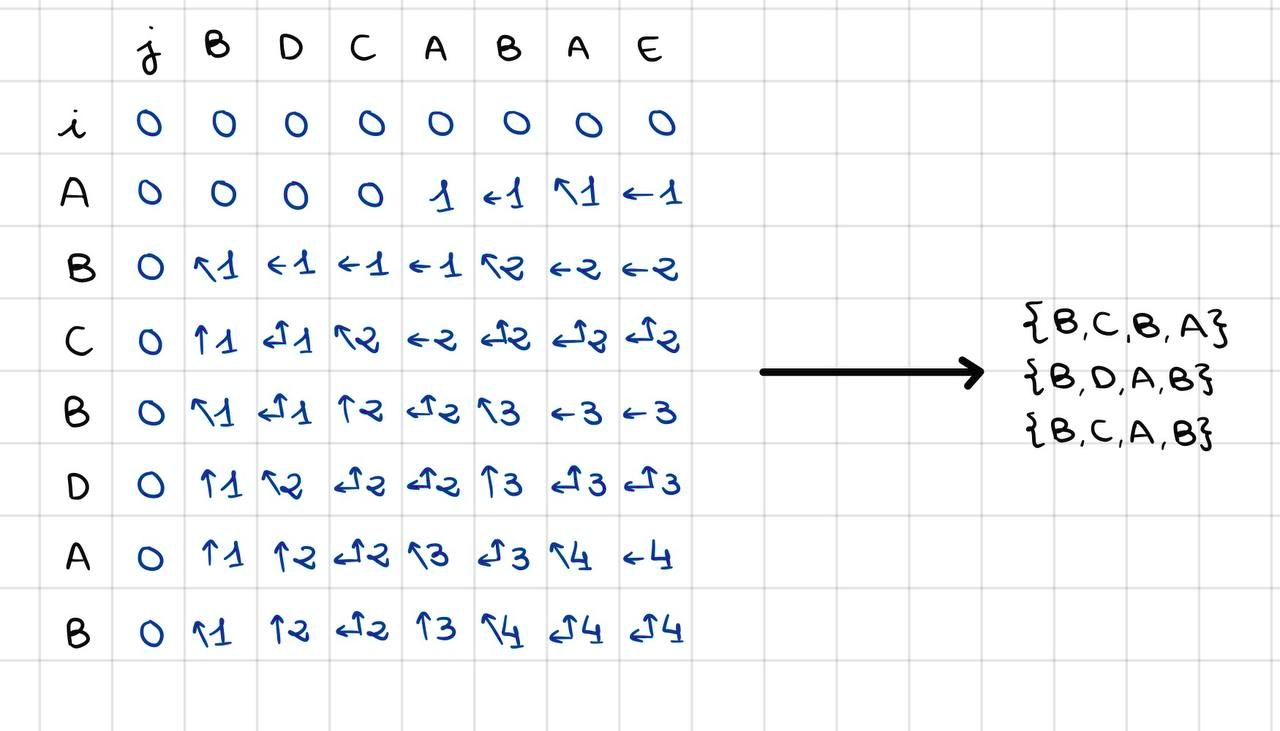
\includegraphics[scale=0.23]{./Ejemplo.png}
	\end{center}
	
	
	\item \textbf{Cálculo de una solución:} Una vez explicado el algoritmo que vamos a usar, mostramos cómo realizamos la entrada de datos en nuestro programa, al igual que la implementación de los 3 pasos descritos anteriormente:
	
	\textbf{1. Entrada de datos}
	\\
	\lstinputlisting[language=C++]{./Code/datos.cpp}
	\textbf{2. Creación e inicialización de la matriz}
	\\
	\lstinputlisting[language=C++]{./Code/inicializacion.cpp}
	\textbf{3. Cálculo de la matriz}
	\\
	\lstinputlisting[language=C++]{./Code/calculo.cpp}
	\textbf{4. Localización del máximo y obtención de la subsecuencia más larga}
	\\
	\lstinputlisting[language=C++]{./Code/maxysub.cpp}
	
	Para el cálculo del \textbf{porcentaje de similitud}, simplemente dividimos el tamaño de la subsecuencia más larga hallada entre el tamaño de cualquiera de las dos cadenas, ya que son de la misma longitud, y multiplicamos el valor del cociente por 100:
	\lstinputlisting[language=C++]{./Code/similitud.cpp}
	
\end{itemize}

\section{Solución}

Una vez expuesto nuestro algoritmo para resolver el problema y su implementación en C++, mostramos los resultados que se nos pedían:

\begin{itemize}
	\item \textbf{1. Secuencias más largas de ambos casos}
	
	\begin{center}
		SECUENCIA MÁS LARGA LETRAS: a b b c d e a b c d z y c c d
		\\
		SECUENCIA MÁS LARGA NÚMEROS: 1 1 0 0 0 0 0 0 1 0 1 0 1 0 1 0 0 1 0 0 0 1 0 0 1 0 0 1 0 0
	\end{center}

	\item \textbf{2. Porcentaje de similitud}
	
	\begin{center}
		PORCENTAJE DE SIMILITUD LETRAS: 88.2353\%
		\\
		PORCENTAJE DE SIMILITUD NÚMEROS: 83.3333\%
	\end{center}

	\item \textbf{3. Matriz de cálculos del primer problema}

	\[
	\begin{matrix}
      &   & a & b & b & c & d & e & a & f & b & c & d & z & x & y & c & c & d \\
      & 0 & 0 & 0 & 0 & 0 & 0 & 0 & 0 & 0 & 0 & 0 & 0 & 0 & 0 & 0 & 0 & 0 & 0 \\
    a & 0 & 1 & 1 & 1 & 1 & 1 & 1 & 1 & 1 & 1 & 1 & 1 & 1 & 1 & 1 & 1 & 1 & 1 \\
    b & 0 & 1 & 2 & 2 & 2 & 2 & 2 & 2 & 2 & 2 & 2 & 2 & 2 & 2 & 2 & 2 & 2 & 2 \\
    b & 0 & 1 & 2 & 3 & 3 & 3 & 3 & 3 & 3 & 3 & 3 & 3 & 3 & 3 & 3 & 3 & 3 & 3 \\
    c & 0 & 1 & 2 & 3 & 4 & 4 & 4 & 4 & 4 & 4 & 4 & 4 & 4 & 4 & 4 & 4 & 4 & 4 \\
    d & 0 & 1 & 2 & 3 & 4 & 5 & 5 & 5 & 5 & 5 & 5 & 5 & 5 & 5 & 5 & 5 & 5 & 5 \\
    e & 0 & 1 & 2 & 3 & 4 & 5 & 6 & 6 & 6 & 6 & 6 & 6 & 6 & 6 & 6 & 6 & 6 & 6 \\
    f & 0 & 1 & 2 & 3 & 4 & 5 & 6 & 6 & 7 & 7 & 7 & 7 & 7 & 7 & 7 & 7 & 7 & 7 \\
    a & 0 & 1 & 2 & 3 & 4 & 5 & 6 & 7 & 7 & 7 & 7 & 7 & 7 & 7 & 7 & 7 & 7 & 7 \\
    b & 0 & 1 & 2 & 3 & 4 & 5 & 6 & 7 & 7 & 8 & 8 & 8 & 8 & 8 & 8 & 8 & 8 & 8 \\
    c & 0 & 1 & 2 & 3 & 4 & 5 & 6 & 7 & 7 & 8 & 9 & 9 & 9 & 9 & 9 & 9 & 9 & 9 \\
    d & 0 & 1 & 2 & 3 & 4 & 5 & 6 & 7 & 7 & 8 & 9 & 10 & 10 & 10 & 10 & 10 & 10 & 10  \\
    x & 0 & 1 & 2 & 3 & 4 & 5 & 6 & 7 & 7 & 8 & 9 & 10 & 10 & 11 & 11 & 11 & 11 & 11\\
    z & 0 & 1 & 2 & 3 & 4 & 5 & 6 & 7 & 7 & 8 & 9 & 10 & 11 & 11 & 11 & 11 & 11 & 11 \\
    y & 0 & 1 & 2 & 3 & 4 & 5 & 6 & 7 & 7 & 8 & 9 & 10 & 11 & 11 & 12 & 12 & 12 & 12\\
    c & 0 & 1 & 2 & 3 & 4 & 5 & 6 & 7 & 7 & 8 & 9 & 10 & 11 & 11 & 12 & 13 & 13 & 13 \\
    c & 0 & 1 & 2 & 3 & 4 & 5 & 6 & 7 & 7 & 8 & 9 & 10 & 11 & 11 & 12 & 13 & 14 & 14 \\
    d & 0 & 1 & 2 & 3 & 4 & 5 & 6 & 7 & 7 & 8 & 9 & 10 & 11 & 11 & 12 & 13 & 14 & 15 
	\end{matrix}
	\]
	
\end{itemize}

\section{Conclusiones}

\begin{itemize}
	\item Si hubiésemos resuelto este problema usando la \textbf{fuerza bruta}, es decir, enumerando todas las subsecuencias comunes existentes, obtendríamos un algoritmo de orden $O(d^n)$, siendo $d$ la longitud de las cadenas.
	\item Gracias a la \textbf{programación dinámica}, evitamos muchos de los cálculos que se harían en \textbf{fuerza bruta}, obteniendo así un algoritmo de \textbf{orden polinomial}, en este caso concretamente $O(n \cdot m)$, siendo $n$ y $m$ las longitudes de las secuencias de entrada.
	\item Obtenemos la \textbf{solución optimal}, cosa que no habríamos logrado con otras técnicas ya vistas como \textbf{Greedy}
	\item También ganamos ventaja respecto a \textbf{Divide y Vencerás}, pues en \textbf{programación dinámica} tenemos problemas que están \textbf{encajados}, por lo que \textbf{no repetimos cálculos}.
	\item Como principal \textbf{inconveniente} de la \textbf{programación dinámica}, se hace un \textbf{gran uso de recursos}, en nuestro caso, la \textbf{memoria} reservada para nuestra \textbf{matriz de cálculos}.
\end{itemize}
\end{document}